\documentclass[goeng, submitted]{thesis}
%\documentclass[goeng, print]{thesis}

\title{%`Hearing the Shapes of Stars:\\
Inverse Problems in Asteroseismology}
%\title{Asteroseismic Inversions of Solar-like and Evolved Stars}%Forward and Inverse Problems in Asteroseismology} % TODO
\author{Earl Patrick Bellinger}
\town{Albany, New York, USA}

\thesisadvisorycommitteea{\textbf{Dr.~ir.~Saskia Hekker}}
\instthesisadvisorycommitteea{\emph{Max-Planck-Institut f\"ur Sonnensystemforschung, G\"ottingen, Germany\\
Stellar Astrophysics Centre, Aarhus University, Denmark}}
\thesisadvisorycommitteeb{\textbf{Prof.~Dr.~Sarbani Basu}}
\instthesisadvisorycommitteeb{\emph{Department of Astronomy, Yale University, New Haven, CT, USA}}
\thesisadvisorycommitteec{\textbf{Prof.~Dr.~Laurent Gizon}}
\instthesisadvisorycommitteec{\emph{Max-Planck-Institut f\"ur Sonnensystemforschung, G\"ottingen, Germany\\
Institut f\"ur Astrophysik, Georg-August-Universit\"at G\"ottingen, Germany}}
\thesisadvisorycommitteed{\textbf{Prof.~Dr.~Ramin Yahyapour}}
\instthesisadvisorycommitteed{\emph{Institut f\"ur Informatik, Georg-August-Universit\"at G\"ottingen, Germany\\
Gesellschaft f\"ur wissenschaftliche Datenverarbeitung mbH G\"ottingen, Germany}}


\refereea{\textbf{Prof.~Dr.~Ramin Yahyapour}}
%\instrefereea{}
\instrefereea{\emph{Institut f\"ur Informatik, Georg-August-Universit\"at G\"ottingen, Germany\\
Gesellschaft f\"ur wissenschaftliche Datenverarbeitung mbH G\"ottingen, Germany}}
\refereeb{\textbf{Prof.~Dr.~Laurent Gizon}}
%\instrefereeb{}
\instrefereeb{\emph{Max-Planck-Institut f\"ur Sonnensystemforschung, G\"ottingen, Germany\\
Institut f\"ur Astrophysik, Georg-August-Universit\"at G\"ottingen, Germany}}



\commissiona{\textbf{Prof.~Dr.~Carsten Damm}}
\instcommissiona{\emph{Institut f\"ur Informatik, Georg-August-Universit\"at G\"ottingen, Germany}}

\commissionb{\textbf{Jun.~Prof.~Dr.~Ing.~Marcus Baum}}
\instcommissionb{\emph{Institut f\"ur Informatik, Georg-August-Universit\"at G\"ottingen, Germany \\
Fakult\"at f\"ur Informatik und Mathematik, Universit\"at Passau, Germany}}

\commissionc{\textbf{Prof.~Dr.~Sarbani Basu}}
%\instcommissionc{}
\instcommissionc{\emph{Department of Astronomy, Yale University, New Haven, CT, USA}}

\commissiond{\textbf{Dr.~ir.~Saskia Hekker}}
%\instcommissiond{}
\instcommissiond{\emph{Max-Planck-Institut f\"ur Sonnensystemforschung, G\"ottingen, Germany\\
Stellar Astrophysics Centre, Aarhus University, Denmark}}

%\commissionc{\textbf{Prof.~Dr.~Laurent Gizon}}
%\instcommissionc{}{\emph{Max-Planck-Institut f\"ur Sonnensystemforschung}}%Only appears with option "additionalreferee"

\submittedyear{2018}
\publicationyear{2018}
\submitteddate{April~5, 2018}
\examinationdate{May~16, 2018}
\isbn{}

\newcommand{\comment}[1]{}
\usepackage[german,english]{babel}

\usepackage[sectionbib]{chapterbib}
\usepackage{natbib}

\usepackage{etoolbox}
\usepackage{calc}
\setlength{\bibhang}{3.3em}

\iffalse
\newcounter{bibcount}
\makeatletter
%\setlength{\bibhang}{3\parindent}
\patchcmd{\@lbibitem}
    {\item[}
    {\item[\hfil\stepcounter{bibcount}{\thebibcount.}}
    {}{}
\setlength{\bibhang}{3.3em}
%\setlength{\leftmargin}{2\parindent}
%\setlength{\itemindent}{-\parindent}
\renewcommand\NAT@bibsetup%
   [1]{\setlength{\leftmargin}{\bibhang}%\setlength{\itemindent}{-\parindent}%
       %\setlength{\itemsep}{\bibsep}\setlength{\parsep}{\z@}}
       }
\makeatother
\fi


%\iffalse
\makeatletter
% patch \@lbibitem to print the current number before the authors
\patchcmd{\@lbibitem}
  {]}
  %{][\theNAT@ctr]}
  %{]\parbox{\widthof{999.}}{\hfill\theNAT@ctr.} }
  %{]\hfil\theNAT@ctr. }
  {]\makebox[\widthof{999.\ }][r]{\theNAT@ctr.\ }\hspace{2mm}}
  {}{}
\makeatother
%\fi

\usepackage{printlen}
\usepackage{color}
\setcounter{tocdepth}{2}%{5}
\setcounter{secnumdepth}{5}
%\setlength{\parindent}{0pt} % Default is 15pt.
%\bibliographystyle{astron}
\usepackage{color}
%\usepackage[svgnames]{xcolor}
\usepackage{xcolor}
\usepackage{framed}
\definecolor{shadecolor}{cmyk}{0.02,0.02,0.02,0.02}%%{named}{LightGray}%{cmyk}{0.088,0.044,0,0}%
\definecolor{xlinkcolor}{cmyk}{1,1,0,0}

\usepackage[bookmarks=false,         % show bookmarks bar?
     pdfnewwindow=true,      % links in new window
     colorlinks=true,    % false: boxed links; true: colored links
     linkcolor=xlinkcolor,     % color of internal links
     citecolor=xlinkcolor,     % color of links to bibliography
     filecolor=xlinkcolor,  % color of file links
     urlcolor=xlinkcolor,      % color of external links
     final=true]{hyperref}

\usepackage{longtable}
\usepackage{import}
\usepackage{physics}
\usepackage{ccaption}

\usepackage{subcaption}

\usepackage{afterpage}
\usepackage{array}
\usepackage{rotating}
\usepackage{pdflscape}

\usepackage{graphicx}	% Including figure files
\usepackage{mathtools}
%\usepackage[fleqn]{amsmath}	% Advanced maths commands
\usepackage{amssymb}	% Extra maths symbols
\usepackage{bm}		    % Bold maths symbols, including upright Greek

\usepackage[makeroom]{cancel}

\usepackage{tikz}
\usetikzlibrary{arrows,positioning,shapes,decorations.markings,patterns,fit}
\usepgflibrary{patterns}
\pgfdeclarepatternformonly{fivepointed stars2}% name
  {\pgfpointorigin}%{\pgfpointorigin}% bottom left
  {\pgfqpoint{5mm}{5mm}}% top right
  {\pgfqpoint{2mm}{2mm}}% tile size
  {% code
   \pgftransformshift{\pgfqpoint{1mm}{1mm}}
   \pgfpathmoveto{\pgfqpointpolar{18}{1mm}}
   \pgfpathlineto{\pgfqpointpolar{162}{1mm}}
   \pgfpathlineto{\pgfqpointpolar{306}{1mm}}
   \pgfpathlineto{\pgfqpointpolar{90}{1mm}}
   \pgfpathlineto{\pgfqpointpolar{234}{1mm}}
   \pgfpathclose%
   \pgfusepath{fill}
}
\pgfdeclarepatternformonly{fivepointed stars3}% name
  {\pgfpointorigin}%{\pgfpointorigin}% bottom left
  {\pgfqpoint{3mm}{3mm}}% top right
  {\pgfqpoint{1.5mm}{1.5mm}}% tile size
  {% code
   \pgftransformshift{\pgfqpoint{1mm}{1mm}}
   \pgfpathmoveto{\pgfqpointpolar{18}{1mm}}
   \pgfpathlineto{\pgfqpointpolar{162}{1mm}}
   \pgfpathlineto{\pgfqpointpolar{306}{1mm}}
   \pgfpathlineto{\pgfqpointpolar{90}{1mm}}
   \pgfpathlineto{\pgfqpointpolar{234}{1mm}}
   \pgfpathclose%
   \pgfusepath{fill}
}

\usepackage{wrapfig}

\usepackage{mathrsfs}
%\usepackage{microtype}

\usepackage{sansmath}

\usepackage[percent]{overpic}
%\usepackage{caption}
%\usepackage[margin=1cm]{caption}
%\captionsetup[table]{skip=10pt}
\usepackage[labelsep=period,labelfont={small,bf,sf}]{caption}
\makeatletter
\renewcommand{\fnum@figure}{\normalsize\bfseries\scshape\sffamily{{Figure \thefigure}}}
\renewcommand{\fnum@table}{\normalsize\bfseries\scshape\sffamily{{Table \thetable}}}
%\renewcommand{\fnum@figure}{\normalsize\scshape{{Figure \thefigure}}}
%\renewcommand{\fnum@table}{\normalsize\scshape{{Table \thetable}}}
\makeatother

\usepackage{needspace}
\usepackage{adjustbox}

%\usepackage{setspace}

%\usepackage{lineno}
%\linenumbers
%\usepackage{enumitem}

%% SI units 
\usepackage{savesym}
\savesymbol{tablenum}
\usepackage{siunitx}
\restoresymbol{SIX}{tablenum}

\usepackage{blkarray}

%\usepackage[numbib]{tocbibind}
%\usepackage{chapterbib}
%\usepackage{etoolbox}
%\patchcmd{\thebibliography}{\chapter*}{\section*}{}{}

\usepackage{pdflscape}
\usepackage{afterpage}
\usepackage{flafter}


\usepackage{eurosym}

%\usepackage{savesym}
%\savesymbol{Sigma}
%\savesymbol{\varv}
\usepackage[sc,osf]{mathpazo} % add possibly `sc` and `osf` options
\usepackage[euler-digits]{eulervm}
%\linespread{1.05}
%\usepackage{breqn}
\DeclareSymbolFont{matha}{OML}{txmi}{m}{it}% txfonts
\DeclareMathSymbol{\varv}{\mathord}{matha}{118}

\usepackage{fancyhdr}
\fancypagestyle{lscape}{% 
\fancyhf{} % clear all header and footer fields 
\fancyfoot[LE]{}
\fancyfoot[LO] {}
\renewcommand{\headrulewidth}{0pt} 
\renewcommand{\footrulewidth}{0pt}}

\def\gridline#1{\vskip6pt\hbox to\hsize{#1}\vskip6pt}

\renewcommand{\mathbf}{\mathbold}
\renewcommand{\boldsymbol}{\mathbold}

\DeclareMathVersion{sans}
\SetSymbolFont{operators}{sans}{OT1}{cmbr}{m}{n}
\SetSymbolFont{letters}{sans}{OML}{cmbrm}{m}{it}
\SetSymbolFont{symbols}{sans}{OMS}{cmbrs}{m}{n}
\SetMathAlphabet{\mathit}{sans}{OT1}{cmbr}{m}{sl}
\SetMathAlphabet{\mathbf}{sans}{OT1}{cmbr}{bx}{n}
\SetMathAlphabet{\mathtt}{sans}{OT1}{cmtl}{m}{n}
\SetSymbolFont{largesymbols}{sans}{OMX}{iwona}{m}{n}


%\let\originalchapter\chapter
\usepackage{quotchap}
%\definecolor{chaptergrey}{cmyk}{1,1,0,0}
\usepackage{epigraph}
\newcommand{\epigraphrulecolor}{white} %xlinkcolor}
\makeatletter
\renewcommand{\@epirule}{{\color{\epigraphrulecolor}\rule[.5ex]{\epigraphwidth}{\epigraphrule}}}
\makeatother
\renewcommand{\textflush}{flushepinormal}
\setlength{\epigraphwidth}{0.85\textwidth}

%\usepackage{titlesec}
\usepackage[raggedright]{titlesec}
\iffalse
\titleformat{\chapter}[display]
  {\normalfont\Huge\bfseries}
  {\chaptertitlename\ \thechapter.}{30pt}{\Huge\normalfont\textit}
\fi
\titleformat{\chapter}[display]
  {\sffamily\fontsize{100}{40}\bfseries}
  {\vspace*{-2cm}\hspace*{5in}\textcolor{gray}{\thechapter}}{10pt}{\raggedright\fontsize{30}{1}\normalfont\textit}%{\Huge\sffamily}%
\titleformat{\section}
  {\normalfont\sffamily\large\bfseries}
  {\thesection}{1em}{}
\titleformat{\subsection}
  {\normalfont\sffamily\normalsize\bfseries}
  {\thesubsection}{1em}{}
\titleformat{\subsubsection}
  {\normalfont\sffamily\normalsize\bfseries\mathversion{sans}}
  {\thesubsubsection}{1em}{}
\titleformat{\paragraph}
  {\normalfont\sffamily\normalsize\bfseries\mathversion{sans}}
  {\theparagraph}{1em}{}
\titleformat{\subparagraph}
  {\normalfont\sffamily\normalsize\bfseries\mathversion{sans}}
  {\theparagraph}{1em}{}
%\newcommand{\sectionbreak}{\clearpage}

%\renewcommand{\thechapter}{\Roman{chapter}}
%\usepackage{chngcntr}% http://ctan.org/pkg/chngcntr
%\counterwithout{section}{chapter}
% make citations sc font
%\newcommand\textlcsc[1]{\textsc{\MakeLowercase{#1}}}
%\makeatletter
%\def\NAT@nmfmt#1{\textlcsc{#1}}
%\makeatother


\newif\ifref
%\reftrue 
\reffalse
\newcommand{\mb}[1]{\ifref\boldmath\textbf{#1}\unboldmath\else #1\fi}

%\newcommand{\colwidth}{0.5\textwidth}
%\newcommand\abs[1]{\left|#1\right|}

%\newcommand\hmmax{0}
%\newcommand\bmmax{0}

%\newcommand{\Teff}{T_{\rm eff}}
%\newcommand{\kmps}{\;{\rm km\;s^{{-}1}}}
%
\newenvironment{absolutelynopagebreak}
  {\par\nobreak\vfil\penalty0\vfilneg
   \vtop\bgroup}
  {\par\xdef\tpd{\the\prevdepth}\egroup
   \prevdepth=\tpd}

\makeatletter
    \clubpenalty10000
    \@clubpenalty \clubpenalty
    \widowpenalty10000
\makeatother

%\usepackage{chngcntr}
%\counterwithout{figure}{chapter}
%\counterwithout{table}{chapter}
%\counterwithout{section}{chapter}

\renewcommand{\baselinestretch}{1.03} 


\newcommand{\half}{\frac{1}{2}}
\newcommand{\Ltwo}{\ell(\ell+1)}
\newcommand{\U}{\frac{4\pi\rho r^3}{m}}
\newcommand{\VV}{\frac{G m \rho}{rP}}
\newcommand{\ddr}{\frac{\text{d}}{\text{d}r}}
\newcommand{\ddx}{\frac{\text{d}}{\text{d}\ln r}}
\newcommand{\ddls}{\frac{\text{d}}{\text{d}\ln s}}
\newcommand{\ddra}[1]{\frac{\text{d} #1}{\text{d}r}}
\newcommand{\ddxa}[1]{\frac{\text{d} #1}{\text{d}\ln r}}
\newcommand{\ddsa}[1]{\frac{\text{d} #1}{\text{d} s}}
\newcommand{\ddlsa}[1]{\frac{\text{d} #1}{\text{d}\ln s}}
\newcommand{\dP}{\frac{\delta P}{P}}
%\newcommand{\dm}{\frac{\delta m}{m}}
\newcommand{\drho}{\frac{\delta \rho}{\rho}}
\newcommand{\dG}{\frac{\delta \Gamma_1}{\Gamma_1}}
\newcommand{\du}{\frac{\delta u}{u}}
%\newcommand{\dY}{\frac{\delta Y}{Y}}
\newcommand{\Gr}{\Gamma_{1,\rho}}
\newcommand{\GP}{\Gamma_{1,P}}
\newcommand{\GY}{\Gamma_{1,Y}}
\newcommand{\Kcr}{K_i^{(c, \rho)}}
\newcommand{\Krc}{K_i^{(\rho, c)}}
\newcommand{\Kcsr}{K_i^{(c^2, \rho)}}
\newcommand{\Krcs}{K_i^{(\rho, c^2)}}
%\newcommand{\KuY}{K_i^{(u,Y)}}
%\newcommand{\KYu}{K_i^{(Y,u)}}
\newcommand{\KGr}{K_i^{(\Gamma_1,\rho)}}
\newcommand{\KrG}{K_i^{(\rho, \Gamma_1)}}
\newcommand{\KGcs}{K_i^{(\Gamma_1,c^2)}}
\newcommand{\KcsG}{K_i^{(c^2,\Gamma_1)}}


\newcommand{\dun}{\frac{\delta u'}{u'}}
\newcommand{\dM}{\delta M}
\newcommand{\dR}{\delta R}
\newcommand{\dMM}{\frac{\dM}{M}}
\newcommand{\dRR}{\frac{\dR}{R}}
\newcommand{\dY}{\delta Y}
\newcommand{\KuY}{K_i^{(u',Y)}}
\newcommand{\KYu}{K_i^{(Y,u')}}
\newcommand{\KuYnop}{K_i^{(u,Y)}}
\newcommand{\KYunop}{K_i^{(Y,u)}}



\definecolor{echelle-yellow}{HTML}{F29559}
\definecolor{echelle-blue}{HTML}{0571b0}
\definecolor{echelle-red}{HTML}{DB4D48}
\definecolor{echelle-black}{HTML}{323031}

\definecolor{turn-orange}{HTML}{B16D41}

\definecolor{diff-blue}{HTML}{0571B0}
\definecolor{diff-red}{HTML}{CA0020}
\definecolor{diff-orange}{HTML}{F97100}
\definecolor{diff-purple}{HTML}{551A8B}

%\makeatletter
\newif\ifhbonecolumn
\hbonecolumntrue
%\makeatother
\newcommand{\colwidth}{\ifhbonecolumn 0.5\linewidth\else \linewidth\fi}
\newcommand{\figsize}{\small}%{\ifhbonecolumn\scriptsize\else\small\fi}%
\newcommand{\figfactor}{\ifhbonecolumn 0.66 \else 1 \fi}
\newcommand{\captwidth}{\ifhbonecolumn 7in \else\colwidth\fi}
\newcommand{\widefigwidth}{\ifhbonecolumn 1.3\linewidth\else\linewidth\fi}
\newcommand{\thinfigstar}{\ifhbonecolumn 0.66\linewidth\else 0.5\linewidth\fi}
\newcommand{\thinfig}{\ifhbonecolumn 0.66\linewidth\else\linewidth\fi}
\newcommand{\bottrim}{\ifhbonecolumn 1.4 \else 1.2 \fi}
\newcommand{\righttrim}{\ifhbonecolumn 0.55 \else 0.45 \fi}
\newcommand{\maybebreak}{\ifhbonecolumn\else\\\fi}



% paper4
\newcommand{\Dnu}{\Delta\nu}
\newcommand{\dnu}{\delta\nu}
\newcommand{\Mo}{\rm{M}_\odot}
\newcommand{\Lo}{\rm{L}_\odot}
\newcommand{\Ro}{\rm{R}_\odot}
%\mathchardef\mhyphen="2D
%\def\gridline#1{\vskip6pt\hbox to\hsize{#1}\vskip6pt}
%\def\fig#1#2#3{\hfill\vbox{\parskip=0pt\hsize=#2
%\includegraphics[width=#2]{#1}\vskip2pt\vtop{\centering
%\footnotesize
%\hsize=#2
%#3\vskip1pt
%}}\hfill}
%\newbox\rotatingbox
%\def\rotatetable{\setbox\rotatingbox=\vbox\bgroup}
%\def\endrotatetable{\egroup
%\rotatebox{90}{\vtop{\unvbox\rotatingbox}}
%}
%\usepackage{aastex6}
\newcommand{\corr}{\mathrm{Corr}}
%\usepackage{deluxetable}
%\renewenvironment{description}[1][0pt]
%  {\list{}{\labelwidth=0pt \leftmargin=#1
%   \let\makelabel\descriptionlabel}}
%  {\endlist}
  
%\defcitealias{2016ApJ...830...31B}{Bellinger \& Angelou et al. \textcolor{black}{(}2016\textcolor{black}{, BA1 hereinafter)} }
\defcitealias{2016apj...830...31b}{Bellinger \& Angelou et al. \textcolor{black}{(}2016\textcolor{black}{, BA1 hereinafter)} }
%\usepackage{lmodern}



\defcitealias{nelder1965simplex}{Nelder--Mead}
\defcitealias{galileo}{Galileo}
\defcitealias{2017apj...839..116a}{Angelou \& Bellinger et al.\ }
\defcitealias{hadamard}{Jacques Hadamard}
\defcitealias{brunoinfinito}{Giordano Bruno}
\newcommand{\mycitet}[1]{\citetalias{#1} (\citeyear{#1})}
\newcommand{\mycitealt}[1]{\citetalias{#1}\citeyear{#1}}

\makeatletter
\newcommand*{\cleartoleftpage}{%
  \clearpage
    \if@twoside
    \ifodd\c@page
      \hbox{}\newpage
      \if@twocolumn
        \hbox{}\newpage
      \fi
    \fi
  \fi
}
\makeatother
%\renewcommand{\cleardoublepage}{\cleartoleftpage}


\usepackage{changepage}

\usepackage{pdfpages}

\emergencystretch 3em

\binoppenalty=9999
\relpenalty=9999

\hyphenation{exo-planets}

\usepackage[bottom,marginal,splitrule,multiple]{footmisc}
%\usepackage{txfonts}

%\allowdisplaybreaks


%%%%%%%%%%%%%%%%%%%%%%
%%% BEGIN DOCUMENT %%%
%%%%%%%%%%%%%%%%%%%%%%
\begin{document}
\label{beginning}
%
\includepdf{thesis_cover.pdf}
\selectlanguage{english}
\maketitle


%{\let\newpage\relax\maketitle}

%\iffalse
%\newpage
%\clearpage
\newpage\thispagestyle{empty}~\newpage
%\thispagestyle{plain}
\thispagestyle{empty}
\vspace*{7cm}
%\vspace*{3.8cm}
%\begin{center}
%    \emph{For the love of Science}
%\emph{``Equipped with his five senses, man explores the universe around him and calls the adventure Science.''} --- Edwin Hubble, 1929
\hspace*{0.5cm}\begin{minipage}[c]{0.5\linewidth}
\epigraph{``\emph{Equipped with his five senses, man explores the universe around him and calls \phantom{``}the adventure Science.}''}{--- Edwin Hubble, 1929}
\end{minipage}
\clearpage


{\hypersetup{linkbordercolor=black,linkcolor=black}
%\begingroup\let\clearpage\relax\tableofcontents\endgroup
%\begingroup\let\clearpage\relax\listoffigures\endgroup
%\begingroup
%\let\clearpage\relax
%\let\newpage\relax
\tableofcontents
%\endgroup
%\newpage%\thispagestyle{empty}~\newpage
%\begingroup
%\let\clearpage\relax
%\let\newpage\relax
\listoffigures
%\endgroup
}

%\clearpage
%\begingroup
%\let\clearpage\relax
%\let\newpage\relax
\chapter*{Summary\markboth{Summary}{Summary}}
\addcontentsline{toc}{chapter}{Summary}
Asteroseismology allows us to probe the internal structure of stars through measurements of their global modes of oscillation. 
Thanks to missions such as the NASA \emph{Kepler} space observatory, we now have high-quality asteroseismic data for nearly $100$ solar-type stars. 
This presents an opportunity to determine the core structures of these stars as well as their ages, masses, radii, and other fundamental parameters. 

This thesis is primarily concerned with two inverse problems. 
The first is to estimate the fundamental parameters of stars from observations using evolutionary arguments. 
This is inverse to the forward problem of simulating the theoretical evolution of a star given the initial conditions. 
We solve this problem using supervised machine learning in Chapter~\ref{chap:ML}. 
We find ages, masses, and radii of stars with uncertainties better than $6\%$, $2\%$, and $1\%$, respectively. 
In Chapter~\ref{chap:statistical}, we furthermore use unsupervised machine learning to quantify how each kind of observation of a star is related to its fundamental parameters. 

The second problem is to infer the structure of a star from its frequencies of pulsation using asteroseismic arguments. 
This is inverse to the forward problem of calculating the theoretical pulsation frequencies of a known stellar structure. 
Solving this problem presents an opportunity to test the quality of stellar evolution models, as we may then directly compare the asteroseismic structure of a star against theoretical predictions. 
We solve this problem in Chapter~\ref{chap:inversion}. 
Applying this technique to the solar-type stars in 16~Cygni, we find that while the structure of the $1.03$ solar mass star 16~Cyg~B is in good agreement with theoretical expectations, the more massive 16~Cyg~A differs in its internal structure from best-fitting evolutionary models. 

These inverse problems are both \emph{ill-posed} in the sense that (I) a solution may not exist within the confines of the current theory; (II) if there is a solution, it may not be unique, as many solutions may be consistent with the data; and/or (III) the solutions may be unstable with respect to small fluctuations in the input data. 
Therefore, care must be put into determining possible solutions and applying regularization where necessary. 

Chapter~\ref{chap:intro} introduces this thesis with the history and theory of stellar structure, evolution, and pulsation; and emphasizes the role that variable star astronomy played in shaping our understanding of stellar evolution. 
It also contains the kernels of stellar structure, an introduction to ill-posed inverse problems, and a discussion of some computational issues for the algorithms used to solve these problems. 

%\endgroup
%\clearpage

%\begingroup
%\let\clearpage\relax
%\let\newpage\relax
\chapter*{Zusammenfassung\markboth{Zusammenfassung}{Zusammenfassung}}
\addcontentsline{toc}{chapter}{Zusammenfassung}
Die Asteroseismologie erlaubt es uns, die innere Struktur der Sterne durch Messungen ihrer globalen Schwingungsmoden zu untersuchen. 
Dank Missionen wie dem Weltraumteleskop \emph{Kepler} der NASA verf\"ugen wir heute \"uber qualitativ hochwertige asteroseismische Daten von fast $100$ sonnen\"ahnlichen Sternen. 
Dies bietet die M\"oglichkeit, das Innere dieser Sterne sowie deren Alter, Masse, Radien und andere fundamentale Parameter zu bestimmen. 

Diese Doktorarbeit besch\"aftigt sich in erster Linie mit zwei inversen Problemen der stellaren Astrophysik. 
Das erste Problem besteht darin, die fundamentalen Parameter eines Sterns aus seinen Beobachtungen mit Hilfe von Argumenten der Sternevolution zu sch\"atzen. 
Dieses Problem ist invers zu dem Vorw\"artsproblem der Simulation der theoretischen Sternentwicklung unter bestimmten Anfangsbedingungen. 
Mit Hilfe von Methoden des \"uberwachten maschinellen Lernens wird dieses Problem in Kapitel~\ref{chap:ML} gel\"ost. 
So ermitteln wir Alter, Masse und Radien mit einer Unsicherheit von weniger als $6\%$, $2\%$ und $1\%$. 
In Kapitel~\ref{chap:statistical} verwenden wir Methoden des un\"uberwachten maschinellen Lernens, um zu quantifizieren wie genau sich die fundamentalen Parametern eines Sterns durch die Kombination verschiedener Arten der Sternbeobachtung bestimmen lassen.

Das zweite Problem besteht darin, die Struktur eines Sterns aus seinen Pulsationsfrequenzen abzuleiten, wobei nur asteroseismische Argumente verwendet werden. 
Dieses Problem ist invers zu dem Vorw\"artsproblem der Berechnung der theoretischen Pulsationsfrequenzen einer bekannten Sternstruktur. 
Die L\"osung dieses Problems bietet die M\"oglichkeit, die Qualit\"at unserer Modelle der Sternentwicklung zu testen, da wir so die asteroseismische Struktur eines Sterns direkt mit theoretischen Vorhersagen vergleichen k\"onnen. 
Dieses Problem wird in Kapitel~\ref{chap:inversion} gel\"ost. 
Wendet man diese Technik auf die beiden sonnen\"ahnlichen Sterne des Systems 16~Cygni an, so stellt man fest, dass die Struktur des $1,03$ Sonnenmassensterns 16~Cyg~B in guter \"Ubereinstimmung mit den theoretischen Vorhersagen ist, w\"ahrend sich der massivere Stern 16~Cyg~A in seiner inneren Struktur von den am besten passenden Evolutionsmodellen unterscheidet. 

Diese inversen Probleme sind im mathematischen Sinne inkorrekt gestellt, sodass (I) eine L\"osung innerhalb der Grenzen der aktuellen Theorie m\"oglicherweise nicht existiert; (II) wenn es eine L\"osung gibt, muss sie nicht eindeutig sein, da viele L\"osungen mit den Daten konsistent sein k\"onnen; und/oder (III) die L\"osungen k\"onnen in Bezug auf kleinere Schwankungen der Ausgangsdaten instabil sein. 
Daher wird viel Sorgfalt darauf verwendet, die Menge der m\"oglichen L\"osungen zu bestimmen und bei Bedarf eine Regularisierung vorzunehmen. 

Kapitel~\ref{chap:intro} leitet diese Arbeit mit der Geschichte und Theorie der Sternstruktur und -evolution ein. Der Schwerpunkt liegt hierbei auf der Theorie der stellaren Pulsationen und wie sie dazu beigetragen hat, unser Verst\"andnis der Sternevolution zu formen. Des Weiteren enth\"alt es Ableitungen der Integralkerne der stellaren Struktur, eine kurze Einf\"uhrung in die mathematisch inkorrekt gestellten inversen Probleme, und eine Diskussion \"uber einige numerische Schwierigkeiten bez\"uglich des maschinellen Lernens und der statistischen Algorithmen die verwendet werden, um diese Probleme zu l\"osen. 

%\endgroup

\subimport{ch1_introduction/}{ch1_introduction.tex}
\subimport{ch2_ML/}{Bellinger.tex}
\subimport{ch3_stats/}{statistical_relations.tex}
\subimport{ch4_inversions/}{Bellinger.tex}

\stepcounter{chapter}
\chapter*{Future Prospects\markboth{Future Prospects}{Future Prospects}}
\addcontentsline{toc}{chapter}{Future Prospects}
\label{chap:prospective}

Though stars are, overall, generally considered to be well-understood, a number of open problems remain in asteroseismology and, more widely, the field of stellar astrophysics as a whole. 
At a basic level, we currently are unable to predict stellar radii from first principles. 
This is due to the fact that we use time-independent one-dimensional theories of convection in evolutionary models---approximations which are controlled by free parameters. 
Properly modelling convection in stellar interiors seems to be among the biggest goals in modern theoretical stellar astrophysics. 
Furthermore, for similar reasons, we generally fail to predict pulsation frequencies of stars, even after making post-hoc corrections for near-surface effects. 

Along similar lines, one of the most basic facts about stars (and astronomical bodies in general) is that they rotate. 
Yet canonical stellar modelling often neglects the effects of rotation, and other similarly `obvious' phenomena such as magnetic fields. 
The very long-term future of research into stars may feature fully 3D magnetohydrodynamical stellar modelling, or even a full treatment of every individual particle that make up the star; however, it is clear that we are far away from that point. 
%Along similar lines, canonical stellar modelling neglects the effects of rotation and magnetic fields.
%This also gives rise to surface effects, which is a nuisance in practically every asteroseismic investigation. 
%Solving convection seems to be the most important  
%Here I will state what I perceive to be some prospects for these areas of research. 
%we can't even predict stellar radii!!!
%The surface term 
%The nature of convective energy transport 
%Fully 3D magnetohydrodynamical stellar modelling 
%Rotation and magnetism 

In terms of the continuation of the research presented in this thesis, there are a few avenues in particular that I intend to explore in the coming months and years: 
\begin{description}
    \setlength{\itemindent}{0pt}
    \item[Structure inversions of more stars.]
    The next step is to apply the technique developed in Chapter~\ref{chap:inversion} to as many stars as possible. 
    This will allow us to determine whether the theory of stellar evolution produces models with the correct interior structures. 
    
    Figures~\ref{fig:phy} and \ref{fig:phy2} show structure inversions for $20$~stars from the \emph{Kepler} LEGACY sample \citep{2017ApJ...835..172L}. 
    The reference models have been constructed under four different assumptions of input physics: with/without diffusion, and with/without convective core overshooting. 
    While some stars show broad agreement throughout their interior with evolutionary models (e.g., KIC~$5184732$), most of the models disagree substantially with the interior structure of the stars. 
    Furthermore, there seems to be no set of input physics considered here that repairs the differences. 
    This indicates that important ingredients may be missing from canonical models of stellar interiors, such as mixing induced by internal rotation. 

%\afterpage{
\begin{figure}
    \centering
    \adjustbox{trim=0cm 1.4cm 0cm 0cm, clip}{%
        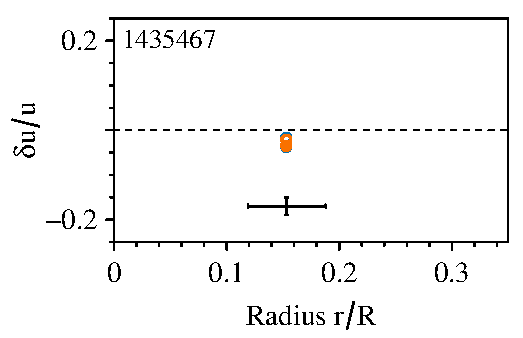
\includegraphics[width=0.55\textwidth]{ch1_introduction/figs/prospective/inversion/1435467.pdf}%
    }%
    \adjustbox{trim=1.6cm 1.4cm 0cm 0cm, clip}{%
        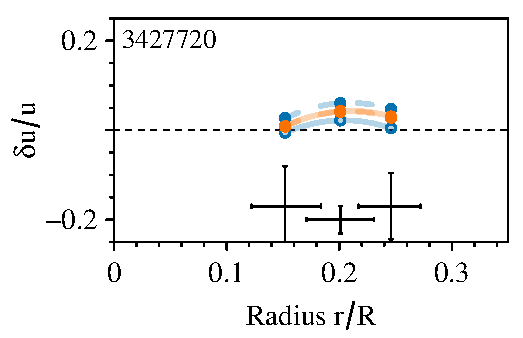
\includegraphics[width=0.55\textwidth]{ch1_introduction/figs/prospective/inversion/3427720.pdf}%
    }\\
    \adjustbox{trim=0cm 1.4cm 0cm 0cm, clip}{%
        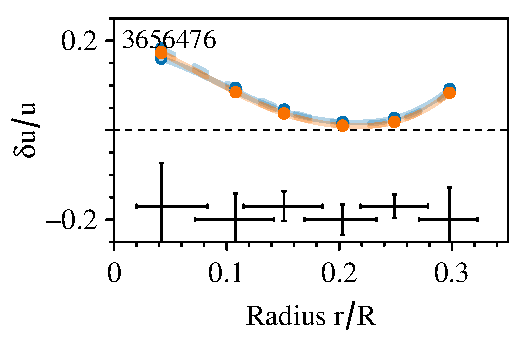
\includegraphics[width=0.55\textwidth]{ch1_introduction/figs/prospective/inversion/3656476.pdf}%
    }%
    \adjustbox{trim=1.6cm 1.4cm 0cm 0cm, clip}{%
        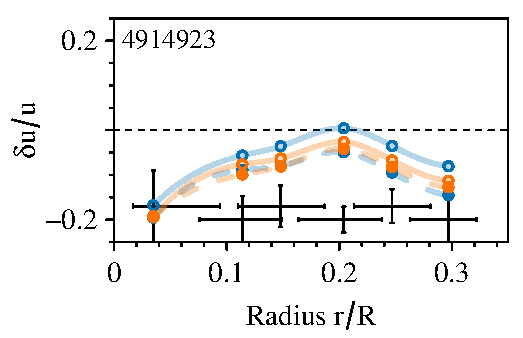
\includegraphics[width=0.55\textwidth]{ch1_introduction/figs/prospective/inversion/4914923.pdf}%
    }\\
    \adjustbox{trim=0cm 1.4cm 0cm 0cm, clip}{%
        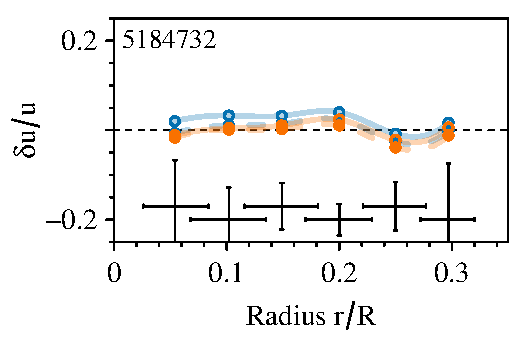
\includegraphics[width=0.55\textwidth]{ch1_introduction/figs/prospective/inversion/5184732.pdf}%
    }%
    \adjustbox{trim=1.6cm 1.4cm 0cm 0cm, clip}{%
        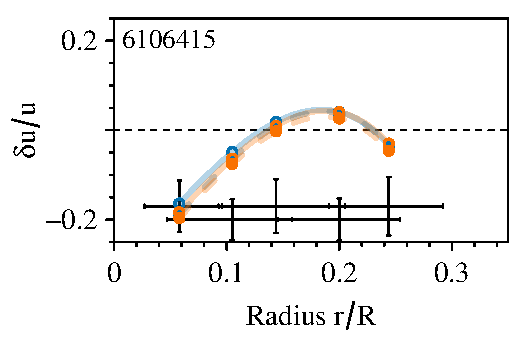
\includegraphics[width=0.55\textwidth]{ch1_introduction/figs/prospective/inversion/6106415.pdf}%
    }\\
    \adjustbox{trim=0cm 1.4cm 0cm 0cm, clip}{%
        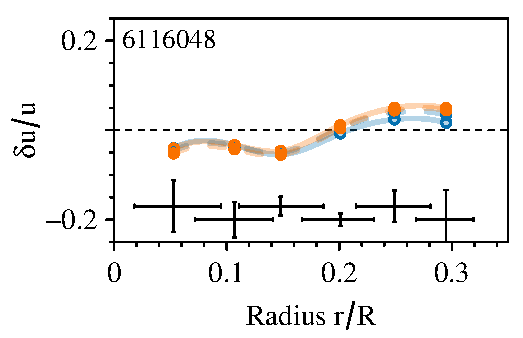
\includegraphics[width=0.55\textwidth]{ch1_introduction/figs/prospective/inversion/6116048.pdf}%
    }%
    \adjustbox{trim=1.6cm 1.4cm 0cm 0cm, clip}{%
        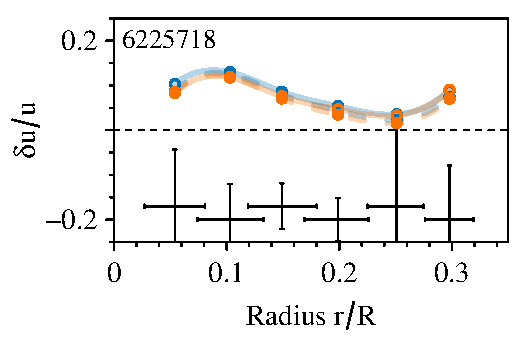
\includegraphics[width=0.55\textwidth]{ch1_introduction/figs/prospective/inversion/6225718.pdf}%
    }\\
    \adjustbox{trim=0cm 0cm 0cm 0cm, clip}{%
        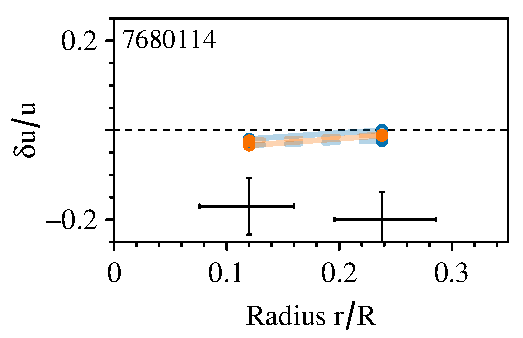
\includegraphics[width=0.55\textwidth]{ch1_introduction/figs/prospective/inversion/7680114.pdf}%
    }%
    \adjustbox{trim=1.6cm 0cm 0cm 0cm, clip}{%
        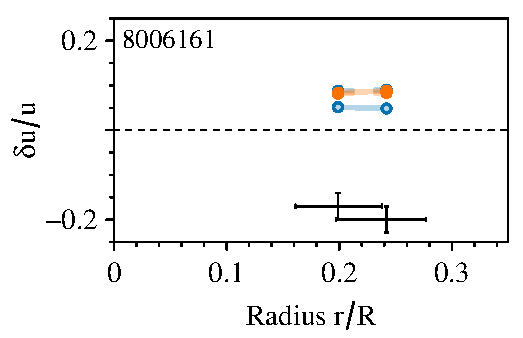
\includegraphics[width=0.55\textwidth]{ch1_introduction/figs/prospective/inversion/8006161.pdf}%
    }%
    \caption[Inversion Zoo]{(Continued in Figure~\ref{fig:phy2}.) \label{fig:phy}}
\end{figure}
\begin{figure}
    \centering
    \adjustbox{trim=0cm 1.4cm 0cm 0cm, clip}{%
        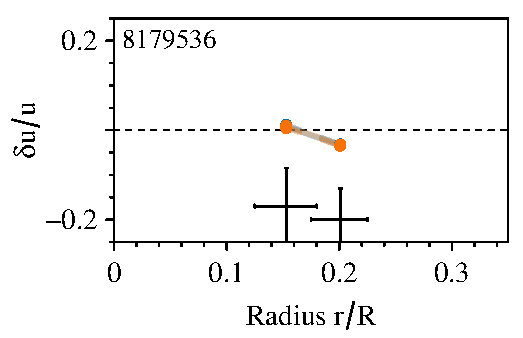
\includegraphics[width=0.55\textwidth]{ch1_introduction/figs/prospective/inversion/8179536.pdf}%
    }%
    \adjustbox{trim=1.6cm 1.4cm 0cm 0cm, clip}{%
        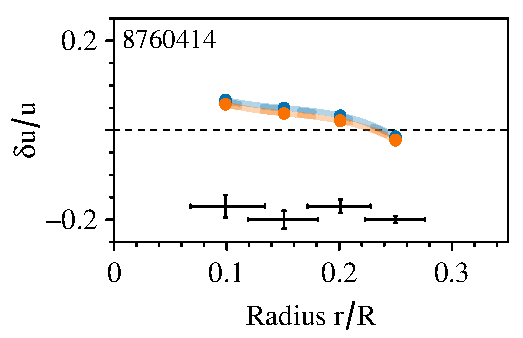
\includegraphics[width=0.55\textwidth]{ch1_introduction/figs/prospective/inversion/8760414.pdf}%
    }\\
    \adjustbox{trim=0cm 1.4cm 0cm 0cm, clip}{%
        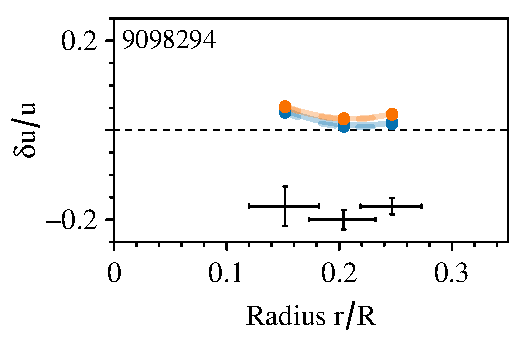
\includegraphics[width=0.55\textwidth]{ch1_introduction/figs/prospective/inversion/9098294.pdf}%
    }%
    \adjustbox{trim=1.6cm 1.4cm 0cm 0cm, clip}{%
        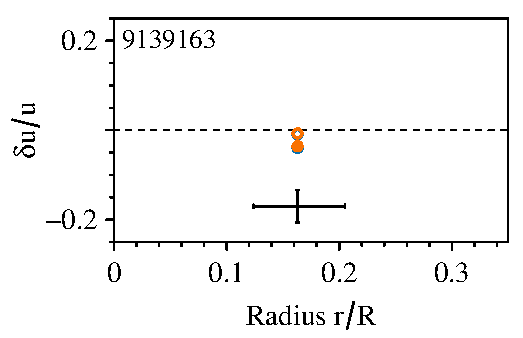
\includegraphics[width=0.55\textwidth]{ch1_introduction/figs/prospective/inversion/9139163.pdf}%
    }\\
    \adjustbox{trim=0cm 1.4cm 0cm 0cm, clip}{%
        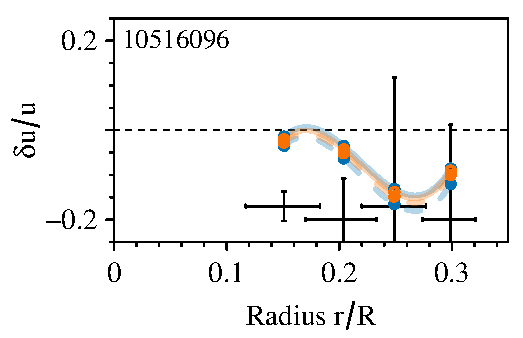
\includegraphics[width=0.55\textwidth]{ch1_introduction/figs/prospective/inversion/10516096.pdf}%
    }%
    \adjustbox{trim=1.6cm 1.4cm 0cm 0cm, clip}{%
        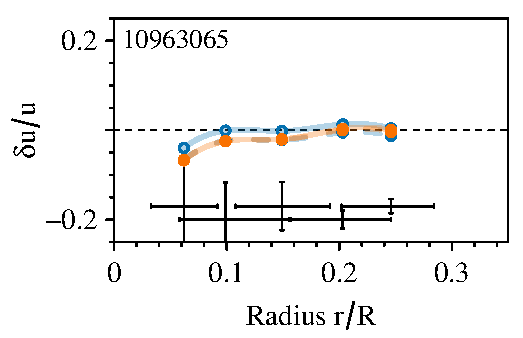
\includegraphics[width=0.55\textwidth]{ch1_introduction/figs/prospective/inversion/10963065.pdf}%
    }\\
    \adjustbox{trim=0cm 1.4cm 0cm 0cm, clip}{%
        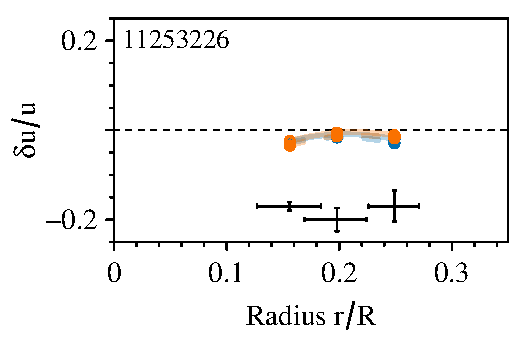
\includegraphics[width=0.55\textwidth]{ch1_introduction/figs/prospective/inversion/11253226.pdf}%
    }%
    \adjustbox{trim=1.6cm 1.4cm 0cm 0cm, clip}{%
        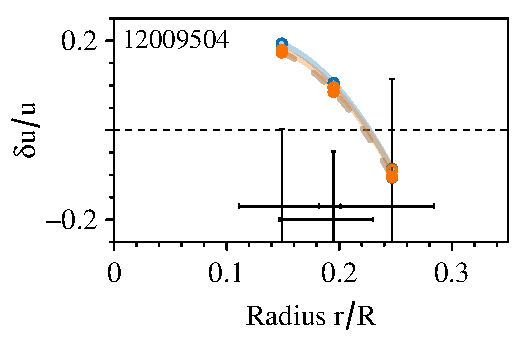
\includegraphics[width=0.55\textwidth]{ch1_introduction/figs/prospective/inversion/12009504.pdf}%
    }\\
    \adjustbox{trim=0cm 0cm 0cm 0cm, clip}{%
        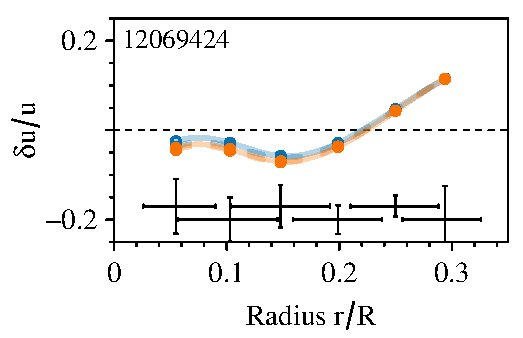
\includegraphics[width=0.55\textwidth]{ch1_introduction/figs/prospective/inversion/12069424.pdf}%
    }%
    \adjustbox{trim=1.6cm 0cm 0cm 0cm, clip}{%
        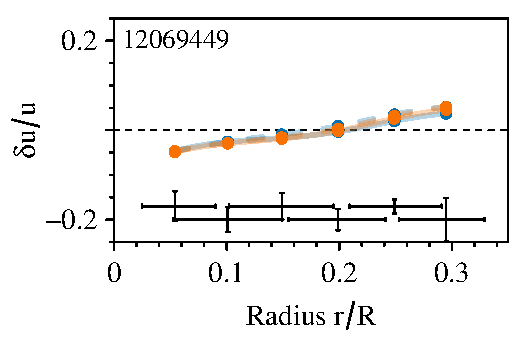
\includegraphics[width=0.55\textwidth]{ch1_introduction/figs/prospective/inversion/12069449.pdf}%
    }%
    \caption[]{(Caption on other page.)
    \label{fig:phy2}}
\end{figure}
%}
\begin{figure}
    \contcaption{Core sound-speed profiles of LEGACY stars compared against stellar models constructed with different physics inputs: with/without diffusion (orange/blue, respectively) and with/without overshooting (filled/open points, respectively). 
    The quantity $\delta u/u$ is the relative difference in the isothermal speed of sound between the model and the star at that location in the stellar interior. 
    The uncertainties of the inversion results and the widths of the corresponding averaging kernels are shown as error bars in the bottom of each panel, and are vertically offset from one another for visibility. }
\end{figure}
    
    This work is soon to be submitted to the Astrophysical Journal. 
    
    
    \item[Evolution inversions of evolved stars.] 
    There have been at least an order of magnitude more detections of solar-like oscillations in evolved stars such as red giants than in main-sequence stars. 
    When combined with kinematic information, determining the ages and chemical compositions of a large number of red giant stars will allow us to reconstruct the history of the Galaxy's development.
    
    In Chapter~\ref{chap:intro} I showed the future evolution of the Sun up through to core helium exhaustion. 
    Current ongoing work is the application of the techniques developed in Chapters~\ref{chap:ML} and \ref{chap:statistical} to these later stages of evolution.  
    
    
    \item[Structure inversions of evolved stars.]
    In this thesis, I analyzed main-sequence solar-like oscillators. 
    After stars leave the main sequence, the $p$-modes in their envelopes mix with the $g$-modes in their deep interiors to give rise to mixed modes of oscillation. 
    Figure~\ref{fig:kernel-evol} shows the evolution of the kernel function for an ${\ell=1}$ mixed mode throughout the sub-giant phase of evolution. 
    After obtaining suitable reference models, for example using the technique mentioned in the previous point, I will invert mixed mode frequencies to determine the core structures of sub-giant and eventually red-giant stars. 
    This presents the exciting prospect for potentially learning more about the deep core structure of another star than we know about our own Sun. 

%\begin{landscape}
\begin{figure}
    \centering
    \hspace*{-1.35cm}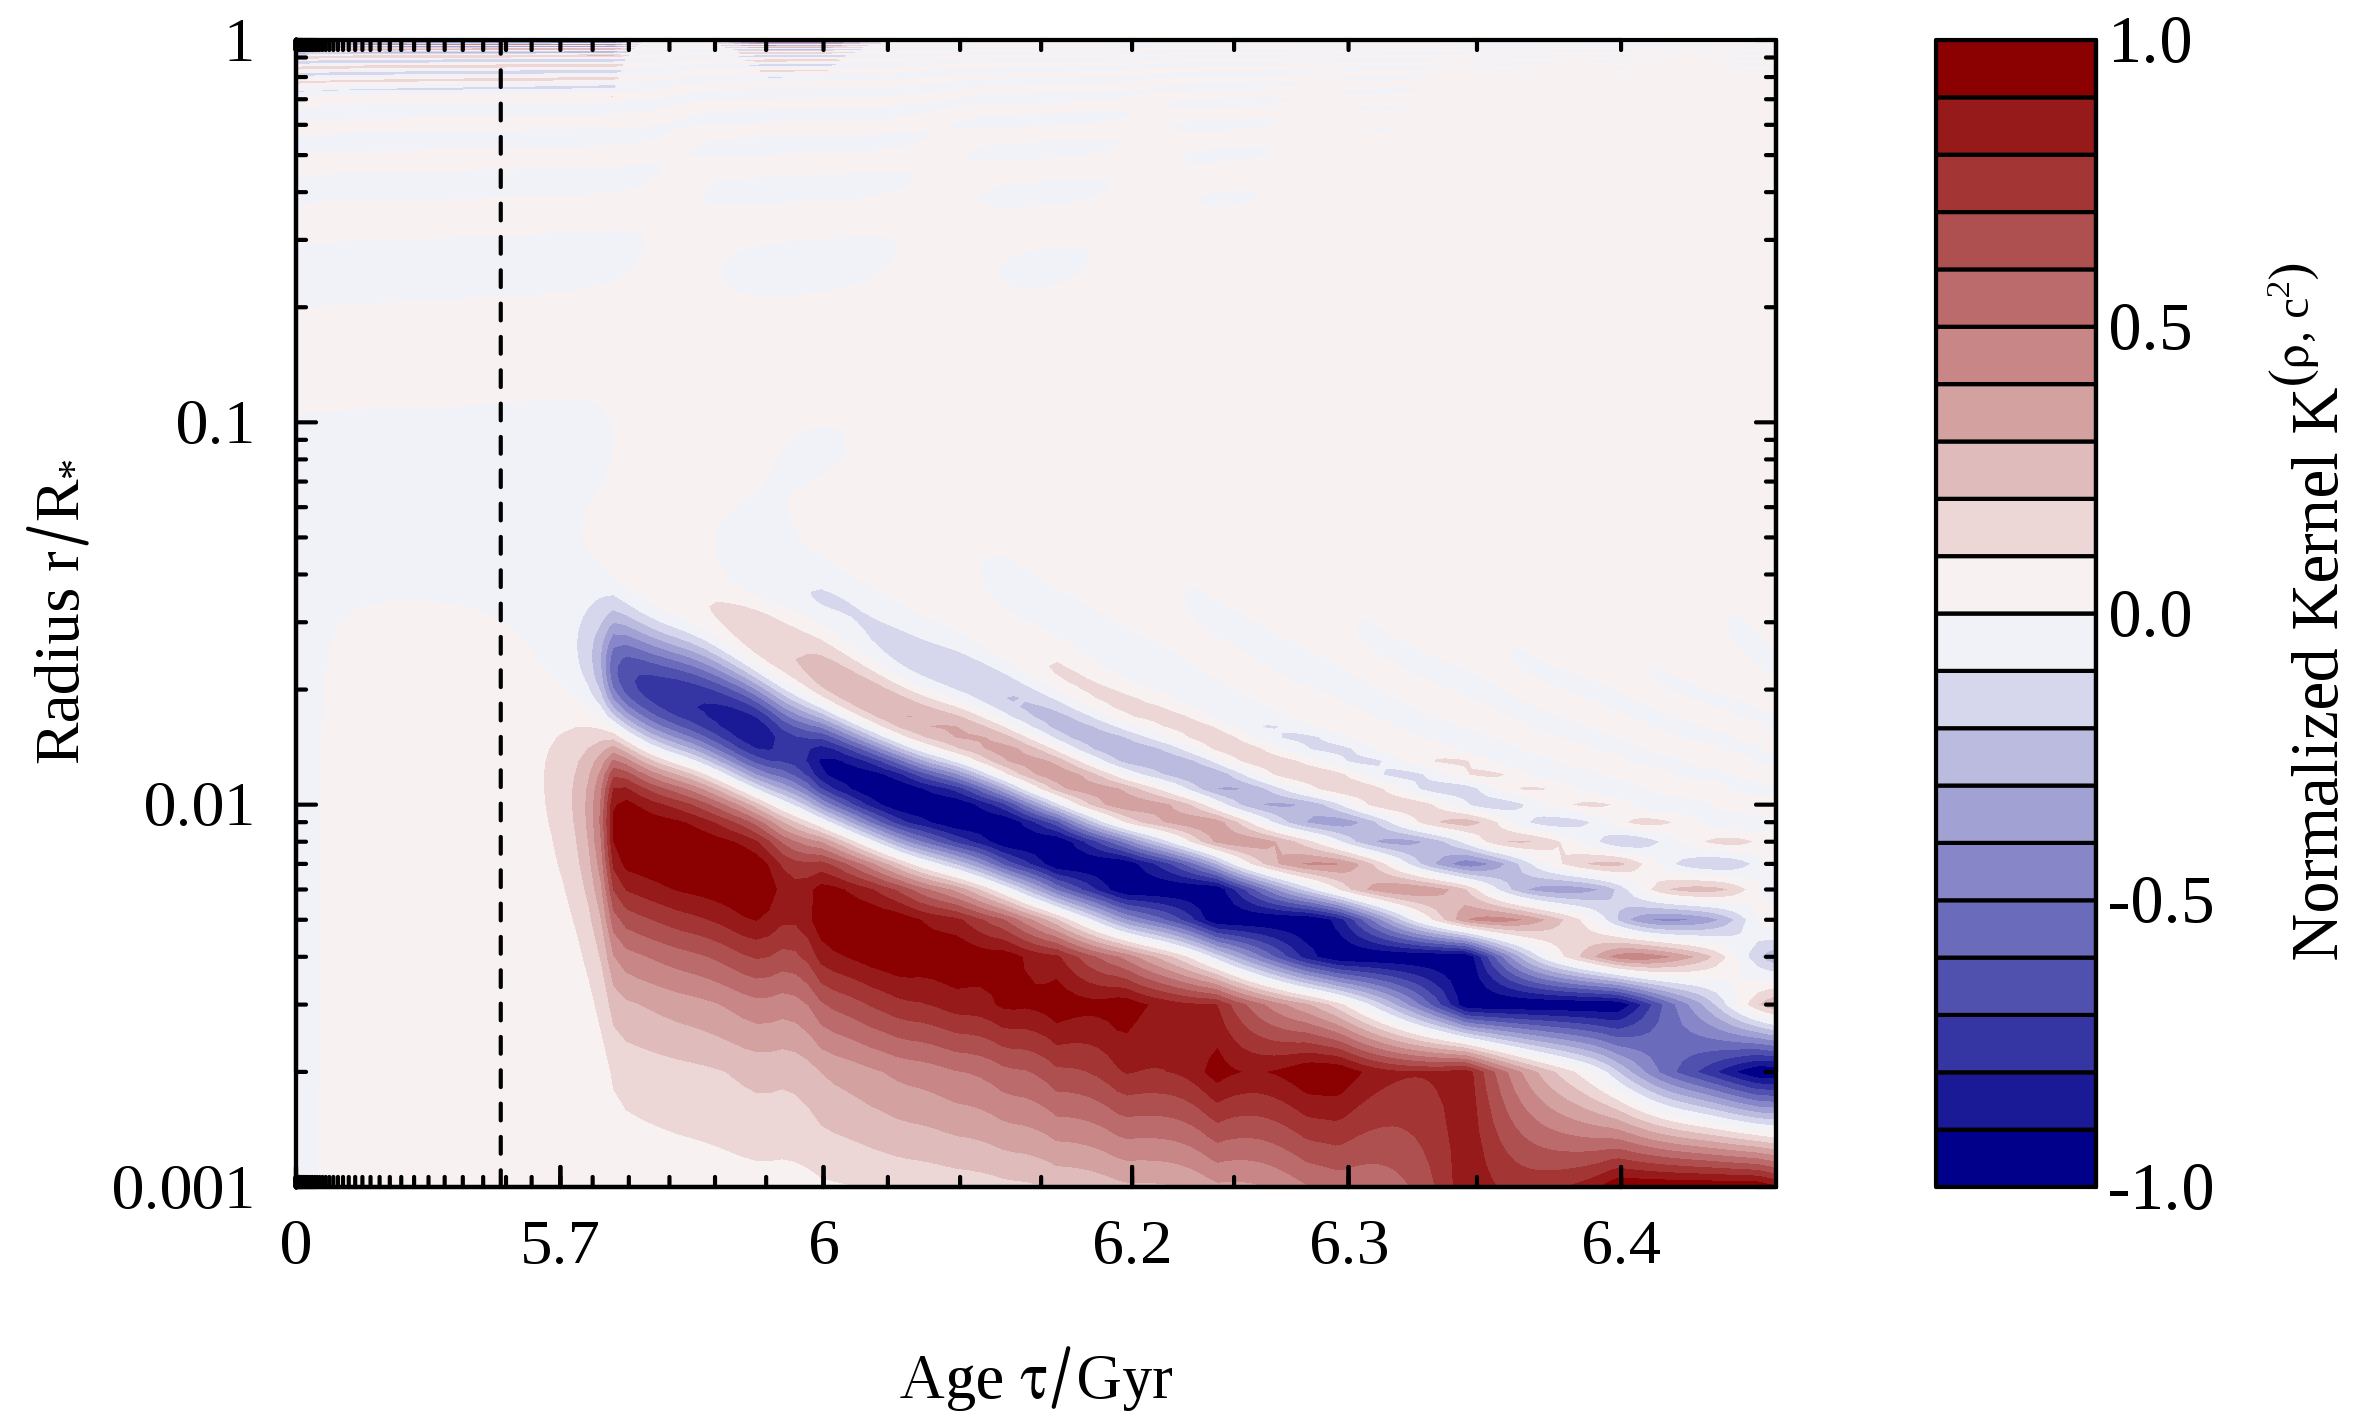
\includegraphics[width=1.2\linewidth]{ch1_introduction/figs/prospective/kernel_evolution-rho-c2-l1_n11.png}
    \caption[Kernel function evolution]{Evolution of the (${\rho, c^2}$) kernel function for the (${\ell=1}, {n=11}$) mode of a ${1.11\; M/M_\odot}$ star. 
        The vertical dashed line shows the end of the main sequence (TAMS). 
        As the mode mixes with a $g$-mode, it develops extreme sensitivity to the deep core structure of the star. 
        \label{fig:kernel-evol}}
\end{figure}
%\end{landscape}
    
    
    \item[Evolution inversions for fundamental constants.]
    A problem of cosmological significance is the measurement of physical constants, and the determination of whether or not they really are constant. 
    The idea of using the Sun to constrain the cosmic variation of the gravitational constant $G$ goes back at least to the time of \citet{Dirac199}. 
    So far, this approach has not been undertaken using other stars. 
    I intend to use the tools discussed in this thesis to measure $G$ as well as other fundamental quantities that impact on stellar evolution and pulsation, such as the fine structure constant \citep[e.g.,][]{2008JCAP...08..010A, 2010AIPC.1269...21C}. 
    Though the Sun is the star with the best data, observations of a large number stars may be able to be combined into a more sensitive tool for these measurements. 
    Furthermore, the Sun's evolution only covers one third of the history of the Universe, and is therefore insensitive to any earlier variations to these quantities. 
\end{description}

In the longer term, there are other prospects that are quite exciting. 
\citet{2014ApJ...782....2L} predicted that $\ell=4$ modes would be observable in 16~Cyg~A and B from \emph{Kepler} data. 
With such data, it would be possible to resolve the sound speed profiles of the observed stars to even shallower layers, which would provide further constraints on theories of the stellar interior. 
However, recent data releases seem not to have produced any such detections. 
%It does not seem that this was the case. 
It does seem feasible within the coming decades that such observations could become available, perhaps through a combination of \emph{Kepler} data with SONG observations \citep{2014RMxAC..45...83A, 2017ApJ...836..142G} and possibly utilizing the forthcoming TESS and PLATO missions. 

In this thesis, I used artificial intelligence to assist in solving problems in stellar astrophysics. 
This is a form of so-called \emph{weak} AI. 
These tools will only get more powerful with the coming decades. 
Eventually, we may have \emph{strong} AI, which will be capable of fully driving scientific research. 
One day, it may be that AI will be able to determine on its own the set of astrophysical laws that are most harmonious with enormous quantities of empirical data. 

%Eventually, I foresee the possibility of AI fully driving scientific research, determining on its own the set of physical laws that are most consonant with enormous quantities of data. 

%In the even longer term, 
%inversions of subgiants 
%inversions of red giants 
%ML of sub and red giants 
%diagnostics from nonradial modes of evolved stars 
%galactic archaeology 
%stars as laboratories to find fundamental constants 
%observations of high degree modes in other stars 
%AI-driven discovery of natural laws 
%\subsection*{Short-Term Prospects}
%\subsection*{Long-Term Prospects}


\chapter*{Bibliography\markboth{Bibliography}{Bibliography}}
\addcontentsline{toc}{chapter}{Bibliography}
\bibliographystyle{thesis.bst}
\setlength{\bibsep}{0.15cm}%0pt plus 1cm}
\renewcommand{\bibsection}{}
\bibliography{thesis}

\chapter*{Publications\markboth{Publications}{Publications}}
\addcontentsline{toc}{chapter}{Publications}
{\bf\large Refereed publications}\\
\begin{enumerate}
    \item \textbf{Bellinger, E.~P.}, Basu, S., Hekker, S., \& Ball, W.: 2017, 
    ``\href{http://adsabs.harvard.edu/abs/2017ApJ...851...80B}{Model-independent Measurement of Internal Stellar Structure in 16~Cygni~A and B}'', 
    \\\emph{The Astrophysical Journal}, 851 (2), 80 
    
    \item \textbf{Bellinger, E.~P.}, Angelou, G.~C., Hekker, S., Basu, S., Ball, W., \& Guggenberger, E.: 2016, 
    ``\href{http://adsabs.harvard.edu/abs/2016ApJ...830...31B}{Fundamental Parameters of Main-Sequence Stars in an Instant with Machine Learning}'', 
    \emph{The Astrophysical Journal}, 830 (1), 20  
    
    \item Angelou, G.~C., \textbf{Bellinger, E.~P.}, Hekker, S., \& Basu, S.: 2017,
    ``\href{http://adsabs.harvard.edu/abs/2017ApJ...839..116A}{On the Statistical Properties of the Lower Main Sequence}'', 
    \emph{The Astrophysical Journal}, 839 (2) 116 (co-first author) 
    
    \item Guggenberger, E., Hekker, S., Basu, S., Angelou, G.~C., \& \textbf{Bellinger, E.~P.}: 2017, 
    ``\href{http://adsabs.harvard.edu/abs/2017MNRAS.470.2069G}{Mitigating the mass dependence in the $\Delta\nu$ scaling relation of red-giant stars}'',
    \emph{Monthly Notices of the Royal Astronomical Society}, 470 (2)%, doi: 10.1093/mnras/stx1253. 
    
    \item Guggenberger, E., Hekker, S., Basu, S., \& \textbf{Bellinger, E.~P.}: 2016
    ``\href{http://adsabs.harvard.edu/abs/2016MNRAS.460.4277G}{Significantly improving stellar mass and radius estimates: A new reference function for the $\Delta\nu$ scaling relation}'', 
    \emph{Monthly Notices of the Royal Astronomical Society}, 461 (2)%, doi: 10.1093/mnras/stw1326. 
    %(\textbf{13 citations})
    
    \item Glover, M., \textbf{Bellinger, E.~P.}, Radivojac, P., \& Clemmer, D.: 2015, 
    ``\href{https://www.ncbi.nlm.nih.gov/pubmed/26192015}{Penultimate Proline in Neuropeptides}'',
    \emph{Analytical Chemistry}, 87 (16), 8466-8472 %, doi: 10.1021/acs.analchem.5b01889. 
    %(\textbf{7 citations})
    
    \item Ji, C., Li, Y., \textbf{Bellinger, E.~P.}, Li, S., Arnold, R., Radivojac, P., \& Tang, H.: 2015, 
    ``\href{https://dl.acm.org/citation.cfm?id=2808750}{A maximum-likelihood approach to absolute protein quantification in mass spectrometry}'', 
    In refereed proceedings of the \emph{6th ACM Conference on Bioinformatics, Computational Biology, and Health Informatics} (pp.~296-305)
    
    \item Ngeow, C.~C., Kanbur, S.~M., \textbf{Bellinger, E.~P.}, Marconi, M., Musella, I., Cignoni, M., \& Lin, Y.~H.: 2012,
    ``\href{http://adsabs.harvard.edu/abs/2012Ap\%26SS.341..105N}{Period-luminosity relations for Cepheid variables: from mid-infrared to multi-phase}'', 
    \emph{Astrophysics and Space Science}, 341 (1), 105-113%, doi: 10.1007/s10509-012-1018-5. 
    %(\textbf{11 citations})
\end{enumerate}

\newpage
\noindent {\bf\large Conference proceedings}\\
\begin{enumerate}
    \item \textbf{Bellinger, E.~P.}, Angelou, G., Hekker, S., Basu, S., Ball, W., \& Guggenberger, E.: 2017,
    ``\href{http://adsabs.harvard.edu/abs/2017EPJWC.16005003B}{Fundamental Parameters in an Instant with Machine Learning: Application to Kepler LEGACY Targets}'', 
    in \emph{Seismology of the Sun and the Distant Stars}, 
    Vol.~60 of \emph{European Physical Journal Web of Conferences}, p.~05003 
    
    \item \textbf{Bellinger, E.~P.}, Wysocki, D., \& Kanbur, S.~M.: 2015,
    ``\href{http://adsabs.harvard.edu/abs/2016CoKon.105..101B}{Measuring amplitudes of harmonics and combination frequencies in variable stars}'', 
    in \emph{Communications from the Konkoly Observatory of the Hungarian Academy of Sciences}, 105 
    
    \item \textbf{Bellinger, E.~P.}, Kanbur, S.~M., \& Ngeow, C.~C.: 2012, 
    ``\href{https://static-content.springer.com/esm/chp\%3A10.1007\%2F978-3-642-29630-7_53/MediaObjects/299986_1_En_53_MOESM13_ESM.pdf}{New insights into the Cepheid PL Relation through the use of multiphase relations}'', 
    in proceedings of the \emph{20th Stellar Pulsations Conference} 
    
    \item \textbf{Bellinger, E.~P.}: 2012,
    ``\href{http://www.ncurproceedings.org/ojs/index.php/NCUR2012/article/view/300}{Multiphase Relations of Magellanic Cloud Cepheids}'', 
    in proceedings of the \emph{2012 National Conference on Undergraduate Research}
    
    \item \textbf{Bellinger, E.~P.}, Kanbur, S.~M., \& Ngeow, C.~C.: 2011,
    ``\href{http://aspbooks.org/custom/publications/paper/451-0311.html}{Multiphase Comparison of Period-Luminosity Relations for Magellanic Cloud Cepheids}'', 
    in proceedings of the \emph{9th Pacific Rim Conference on Stellar Astrophysics}, 451 (311)
    
    \item Hekker, S., Elsworth, Y., Basu, S., \& \textbf{Bellinger, E.~P.}: 2017,
    ``\href{http://adsabs.harvard.edu/abs/2017EPJWC.16004006H}{Evolutionary states of red-giant stars from grid-based modelling}'', 
    in \emph{Seismology of the Sun and the Distant Stars}, 
    Vol.~160 of \emph{European Physical Journal Web of Conferences}, p.~05003 
    
    \item Reyner, S., \textbf{Bellinger, E.~P.}, \& Kanbur, S.~M.: 2012,
    ``\href{https://static-content.springer.com/esm/chp\%3A10.1007\%2F978-3-642-29630-7_53/MediaObjects/299986_1_En_53_MOESM44_ESM.pdf}{The approximation of RR Lyrae and eclipsing binary light curves using cubic polynomials}'', 
    in proceedings of the \emph{20th Stellar Pulsations Conference}
\end{enumerate}
    
    
\vspace{2\baselineskip}

\noindent {\bf\large Technical reports}\\
\begin{enumerate}
    \item \textbf{Bellinger, E.~P.}, Conner, D., Mittman, D., Magee, K., \& Heventhal, B.: 2012,
    ``\href{https://trs.jpl.nasa.gov/handle/2014/43122}{CASSIUS: the Cassini Uplink Scheduler}'', 
    \emph{JPL: NASA}, hdl:2014/43122
\end{enumerate}


\chapter*{Acknowledgements\markboth{Acknowledgements}{Acknowledgements}}
\addcontentsline{toc}{chapter}{Acknowledgements}
This thesis represents the culmination of my, by now, nearly ten-year-long fascination with variable stars, which began way back in my first year of university. 
It would have been all but impossible to chase this dream without the support of many individuals. 
I would like now to give thanks to all those who have supported me on this journey. 

I would first like to thank my doctoral advisors, Dr.\ ir.\ Saskia Hekker and Prof.\ Dr.\ Sarbani Basu, for their advice, guidance, and good ideas over the past three years. 
I appreciate the amount they pushed me to make this thesis what it is, and I look back with amazement at all the things I have been given the opportunity to learn about. 
I am proud of the hard work that they encouraged from me, and I look forward to continued collaboration in the future. 

During my studies, I have had the great fortune of being able to lean on the expertise of two post-docs, Dr.\ George Angelou and Dr.\ Warrick Ball. 
Without their help, I would have surely been stuck in the dark for far longer than I was. 
I want to especially thank George for teaching me about stellar evolution, and to thank Warrick for teaching me about kernels. 
I hope we will continue to collaborate long into the future! 

Next I want to thank the SAGE Group at the Max Planck Institute for Solar System Research and the Department of Astronomy at Yale University for hosting me over these three years. 
I have greatly enjoyed my stays, the exchange of ideas, and the numerous friendships that I've made in these places. 
I also thank the IMPRS scientific coordinator, Dr.\ Sonja Schuh, and the staff at both Yale University and the MPS for all their assistance. 
I especially want to thank the IMPRS Student Group, which makes it easy for anyone from anywhere to fit in and make friends. 
I also thank Dr.\ Timo Reinhold for his assistance with the German language. 

Special thanks go to the Director of the Max Planck Institute for Solar System Research, Prof.\ Dr.\ Laurent Gizon; the Director of the GWDG, Prof.\ Dr.\ Ramin Yahyapour; and the Dean of Computer Science, Prof.\ Dr.\ Jens Grabowski for helping me to enroll into the 
%Sparing the long story, it was somewhat unclear for a time whether my graduate studies would actually be able to continue. 
%These three saved me by helping me to enroll into the 
G\"ottingen Ph.D.\ Programme in Computer Science. 
Additionally, I thank the remaining members of the examination board, Prof.\ Dr.\ Carsten Damm and Jun.\ Prof.\ Dr.\ Ing.\ Marcus Baum, for agreeing to examine this thesis. 

I thank the National Physical Science Consortium for their very generous support in the form of a graduate fellowship over five years of my graduate studies. 
I also thank Dr.\ Judith E.\ Devaney Terrill for selecting me for the NPSC Fellowship, for hosting me at NIST for two summers, and especially for always encouraging a strong scientific mindset. 

I have had the privilege and honor of working with and (co-)supervising several wonderful students over the course of my graduate studies. 
I want to acknowledge: Felix Ahlborn (now a Ph.D.\ student at the Max Planck Institute for Astrophysics), Kenny Roffo (now employed at the NASA Jet Propulsion Laboratory and pursuing graduate studies at Johns Hopkins University), Marc Hon (finishing up his Ph.D.\ at the University of New South Wales in Sydney, Australia), and Alejandra Perea Rojas (in the midsts of applying to prestigious universities). 
I'm proud of you all - keep up the great work! 

At the Max Planck Institute for Solar System Research, we started a band called MegaGau{\ss} that practices every Monday evening and provides a much needed reprieve from the sometimes rollarcoaster-like nature of academia. 
I want to thank everyone who has played and participated over the last three years and over the many gigs we had; this list includes over twenty people! 
With no guarantee of completeness, the band included 
Abbey Ingram, %(flute),
Alessandro Cilla, %(guitar/vocals),
Bastian Proxauf, % (trombone),
Carla Wiles, % (ukulele/vocals),
ChiJu Wu, % (trumpet),
Daniel Maase,
David Marshall, % (clarinet/saxophone),
Fatima Kahil, % (acoustic guitar),
Felix Mackebrandt, % (percussion),
Hans Huybrighs, % (electric guitar),
Holly Waller, % (bass guitar),
Katja Karmrodt, % (vocals),
Kenny Roffo, % (electric guitar),
Nils Gottschling, % (bass guitar),
Robin Thor, % (keyboard),
Sudharshan Saranathan, % (vocals),
Dr.\ Ankit Barik, % (vocals),
Dr.\ David Martin Belda, % (guitar),
Dr.\ Emanuele Papini, % (keyboard),
Dr.\ James Kuszlewicz, % (guitar/mandolin),
Dr.\ Keaton Bell, % (guitar), and
Dr.\ Theodosis Chatzistergos, and
Dr.\ Vera Dobos. % (classical guitar). % (guitar). 
Special thanks go out to my ``other half'' of the rhythm section, Helge Mi{\ss}bach, without whom there would have been no band! 

I want to take this opportunity to thank some of the teachers who have encouraged and inspired me over the years. 
This list includes my high school English, history, and physics teachers: Mr.\ Nelson, Mr.\ Kaufman, Mr.\ Battisti; and several of my college computer science professors: Prof.\ Vampola, Prof.\ Graci, and Prof.\ Dr.\ Early. 

To my `cohort' in the IMPRS school, Alessandro Cilla and Fatima Kahil, and to my other graduate student friends as well: best of luck with finishing your studies! 
To my friend K.\ Casey Shea, thank you for making this amazing thesis cover design for me! 
To all of my dear friends whom I have made over these years of study, thank you for making this journey more enjoyable than it certainly could have been. 
%I also want to acknowledge several of my good friends who have made this journey more enjoyable than it certainly could have been. 
%With fear of leaving out many names: to  Colin McNamara, Madison Van Kuren, Crystal Blakenbaker, David Greco, Dominick Dickerson, %Kenneth Malloy, Thomas Miller, Alysha Taggart, Brandine Jardine, Sean McNamara, 
%Abigail Kleinsmith, Andy Buchmann, Justin M.\ Grimes, Valerie Lazalier, and
%Hussein Mohsen, Jaimie Murdoch, 
%Blake Patrick Coleman. %, %Allen Davis, Mayukh Panja, and Dr.\ Ivan Milic. %to Allen Davis, Lily Zhao, Valentina Kallina, Mayukh Panja, and Dr.\ Ivan Milic; 
%With fear of leaving out many names: to Colin McNamara, Madison Van Kuren, Crystal Blakenbaker, David Greco, and Dominick Dickerson; to Kenneth Malloy, Thomas Miller, Alysha Taggart, and Brandine Jardine; to Sean McNamara, Abigail Kleinsmith, Andy Buchmann, and Justin M.\ Grimes; to Valerie Lazalier, Hussein Mohsen, Jaimie Murdoch, and Blake Patrick Coleman; %to Allen Davis, Lily Zhao, Valentina Kallina, Mayukh Panja, and Dr.\ Ivan Milic; 
%to Carla Wiles. 
Special thanks go to Carla Wiles, for many things, including her support and her valued opinions on all the aesthetic aspects of this thesis. 

I want to thank my family for their unwavering support in my choice to study something as academic as the distant stars. 
I thank my mother Patricia, my father Paul, my sister Bobbie Lee, her partner Johnny, my brother Sean, my sister-in-law Valentina, my niece Nia, my nephews Rashay and Darius, and my step-parents Ron and Nina. 

Last, and certainly not least, I dedicate this thesis to my mentor, Prof.\ Dr.\ Shashi M.\ Kanbur, who has continuously and actively encouraged me over the past decade to pursue my ``academic dreams.'' 
Thank you, Shashi, for always being there for me, and for showing me the light of variable stars. 
 

\chapter*{Curriculum vitae\markboth{Curriculum vitae}{Curriculum vitae}}
\addcontentsline{toc}{chapter}{Curriculum vitae}
\iffalse
\begin{wrapfigure}[0]{r}{0.3\textwidth} 
    \centering
    \vspace*{-2.95cm}
    \tikz\node[circle,draw,minimum size=3.5cm,
                path picture={
                    \node at (path picture bounding box.center){
                        \includegraphics[width=3.5cm,height=3.5cm]{avatar2.jpg}
                    };
                }]{};
    %\includegraphics[width=100pt]{avatar2.jpg}
\end{wrapfigure}
\fi

{\Large\textbf{Earl Patrick Bellinger}}
%\section*{Earl Patrick Bellinger}

%\vspace*{0.5cm}
  % Education
  \section*{\sc\underline{Education}}
  \vspace*{-2mm}
  %\vspace*{-1cm}\par\noindent\rule{\textwidth}{0.4pt}\vspace{1cm}

%  \textbf{Indiana University}, Bloomington, IN, USA \hfill \textbf{Fall 2012 -- Present}\vspace{1mm}\\
%  Ph.D.~Student in Computer Science \\
%  M.Sc.~Computer Science with a specialization in Bioinformatics \hfill (completed December 2014)\\
  %\textbf{Ph.D.~Astrophysics}, International Max Planck Research School \hfill (\emph{expected 2018})\vspace{1mm}\\
  %\textbf{Ph.D.~Theoretical Astrophysics}, University of G\"ottingen \hfill (\emph{expected 2018})\vspace{1mm}\\
  \noindent\textbf{Ph.D.~Candidate}, Institute of Computer Science, University of G\"ottingen\\ %\hfill 2015--2018\\
  International Max Planck Research School for Solar System Science\\
  Fellow of the National Physical Science Consortium\vspace{2mm}\\%\\
  %Thesis: \emph{\hyperref[beginning]{Inverse Problems in Asteroseismology}}\vspace{2mm}\\
  \noindent\textbf{M.Sc.~Computer Science}, Indiana University Bloomington, USA \hfill 2014\\
  Fellow of the National Physical Science Consortium \\
  %Minor in Bioinformatics \\
  GPA: 3.95/4.0\vspace{2mm}\\
  \textbf{B.Sc.~Applied Mathematics}, SUNY Oswego, NY, USA \hfill 2012\\
  \textbf{B.Sc.~Computer Science}, \emph{ibid.} \hfill 2012\\
  Presidential Scholar\\
  Honors Thesis: \emph{Multiphase Relations of Magellanic Cloud Cepheids} \\
  GPA: 3.81/4.0 (\emph{summa cum laude}, ranked \#1 in Computer Science)

  % Experience
  \section*{\sc\underline{Research Positions}}
  \vspace*{-2mm}
  %\vspace*{-1cm}\par\noindent\rule{\textwidth}{0.4pt}\vspace{1cm}
  
  \noindent\textbf{Max Planck Institute for Solar System Research} \emph{(Germany)} \hfill 2015 -- 2018\\
  Doctoral Candidate, Stellar Ages \& Galactic Evolution Group \vspace{1mm}\\
  \textbf{Yale University} \emph{(USA)} \hfill 2016 -- 2017\\
  Visiting Assistant in Research, Department of Astronomy\vspace{1mm}\\
  \textbf{Indiana University} \emph{(USA)} \hfill 2013 -- 2015\\
  Research Assistant, School of Informatics \& Computing \vspace{1mm}\\
  \textbf{NIST Information Technology Laboratory} \emph{(USA)} \hfill 2013 -- 2014\\
  Guest Researcher, Scientific Applications and Visualization Group \vspace{1mm}\\
  \textbf{National Center of Sciences} \emph{(Japan)} \hfill 2013\\
  Research Student, National Institute of Informatics \vspace{1mm}\\
  \textbf{NASA Jet Propulsion Laboratory} \emph{(USA)} \hfill  2012\\
  SURF Fellow, Cassini Mission to Saturn \vspace{1mm}\\
  \textbf{Federal University of Alagoas} \emph{(Brazil)} \hfill 2011\\
  REU Student, Institute of Physics\vspace{1mm}\\
  \textbf{Federal University of Santa Catarina} \emph{(Brazil)} \hfill 2010\\
  REU Student, Department of Physics
  
  % Teaching experience
  \section*{\sc\underline{Teaching Positions}}
  \vspace*{-2mm}
  \textbf{Yale University} \hfill Spring 2017\\
  Teaching Assistant, Department of Astronomy\vspace{1mm}\\
  \textbf{University of G\"ottingen} \hfill Summer 2016\\
  Assistant, Institute for Astrophysics \vspace{1mm}\\
  \textbf{Indiana University} \hfill Fall 2012\\
  Associate Instructor, School of Informatics \& Computing\vspace{1mm}\\
  \textbf{SUNY Oswego} \hfill Fall 2010\\
  Seminar Leader, Honors Department
  
  \vspace*{-4.2mm}
  \section*{{\sc\underline{Selected Talks}} \hfill {\normalsize\normalfont $^{\scriptscriptstyle\bigstar}$\emph{invited}}}
  \vspace*{-2mm}
  \noindent $^{\scriptscriptstyle\bigstar}$\textbf{Stellar Astrophysics Centre Seminar} (Aarhus, Denmark) \hfill{2018} \\
  \hphantom{$^{\scriptscriptstyle\bigstar}$}``\emph{Determining stellar structure with asteroseismology using novel techniques}''
  
  \vspace{1mm}
  \noindent \hphantom{$^{\scriptscriptstyle\bigstar}$}\textbf{TESS/Kepler Asteroseismic Science Consortium} (Aarhus, Denmark) \hfill{2018} \\
  \hphantom{$^{\scriptscriptstyle\bigstar}$}``\emph{Testing stellar physics with asteroseismic inversions of solar-type stars}''

  \vspace{1mm}
  \noindent $^{\scriptscriptstyle\bigstar}$\textbf{Madison Seminar} (University of Wisconsin--Madison, USA) \hfill{2017} \\
  \hphantom{$^{\scriptscriptstyle\bigstar}$}``\emph{From Starlight to Stellar Ages with Asteroseismology}''
  
  \vspace{1mm}
  \noindent \hphantom{$^{\scriptscriptstyle\bigstar}$}\textbf{Rocks \& Stars II} (Max Planck Institute, G\"ottingen, Germany) \hfill{2017} \\
  \hphantom{$^{\scriptscriptstyle\bigstar}$}``\emph{The Seismic Structures of Solar-Type Stars}''
  
  \vspace{1mm}
  \noindent \hphantom{$^{\scriptscriptstyle\bigstar}$}\textbf{ERES-III} (Yale University, New Haven, CT, USA) \hfill{2017} \\
  \hphantom{$^{\scriptscriptstyle\bigstar}$}``\emph{Fundamental Parameters of Exoplanet Host Stars with Asteroseismology}''
  
  \vspace{1mm}
  \noindent $^{\scriptscriptstyle\bigstar}$\textbf{Science Today} (Public talk at SUNY Oswego, NY, USA) \hfill{2017} \\
  \hphantom{$^{\scriptscriptstyle\bigstar}$}``\emph{A Look Inside the Private Lives of Stars}''
  
  \vspace{1mm}
  \noindent $^{\scriptscriptstyle\bigstar}$\textbf{Red Giant Modeling Workshop} (G\"ottingen, Germany) \hfill{2016} \\
  \hphantom{$^{\scriptscriptstyle\bigstar}$}``\emph{Fundamental Stellar Parameters in an Instant with Machine Learning}''
  
  \vspace{1mm}
  \noindent \hphantom{$^{\scriptscriptstyle\bigstar}$}\textbf{RR Lyrae} (Visegr\'ad, Hungary) \hfill{2015} \\
  \hphantom{$^{\scriptscriptstyle\bigstar}$}``\emph{Resolving Combination Frequency Amplitudes of Multimode Pulsators}''
  
  \vspace{1mm}
  \noindent \hphantom{$^{\scriptscriptstyle\bigstar}$}\textbf{American Astronomical Society} (Seattle, WA, USA) \hfill{2015} \\
  \hphantom{$^{\scriptscriptstyle\bigstar}$}``\emph{Optimal Model Discovery of Periodic Variable Stars}''
  
  \vspace{1mm}
  \noindent $^{\scriptscriptstyle\bigstar}$\textbf{Delhi Workshop on Variable Stars} (Delhi, India) \hfill{2015} \\
  \hphantom{$^{\scriptscriptstyle\bigstar}$}``\emph{Calibrating the Cepheid Distances to the Magellanic Clouds}''
  
  \vspace{1mm}
  \noindent $^{\scriptscriptstyle\bigstar}$\textbf{Kerala Workshop on Stellar Astrophysics} (Kerala, India) \hfill{2014} \\
  \hphantom{$^{\scriptscriptstyle\bigstar}$}``\emph{Automated Supervised Classification of Variable Stars}''
  
  
  
  
  
  \vspace*{-4.2mm}
  % Honors and Awards
  \section*{\sc\underline{Honors \& Awards}}
  \vspace*{-2mm}
  Stellar Astrophysics Centre Postdoctoral Fellowship \hfill 2018 -- 2021\vspace{1mm}\\
  National Physical Science Consortium Graduate Fellowship    \hfill 2012 -- 2017\vspace{1mm}\\
  SUNY Oswego Presidential Scholarship                        \hfill 2008 -- 2012\vspace{1mm}\\
  Oebele Van Dyk Outstanding Computer Science Senior Award    \hfill 2012\vspace{1mm}\\
  SUNY Chancellor's Award %for Student Excellence
  \hfill 2012\vspace{1mm}\\
  SUNY Oswego Student/Faculty Collaborative Challenge Grant   \hfill 2011%\vspace{1mm}\\
  %Robert Brian Ellis Scholarship
  %\hfill \textbf{2011}\vspace{1mm}\\
  %New York State Federation of Home Bureau Scholarship        \hfill \textbf{2011}\vspace{1mm}\\
  %NSF IRES / SUNY Oswego Global Laboratory Scholarship        \hfill 2010, 2011\vspace{1mm}\\
  %SMART Grant                                                 \hfill 2010, 2011\vspace{1mm}\\
  %Academic Competitiveness Grant                              %\hfill \textbf{2008}\vspace{1mm}\\
   

\end{document}
